\documentclass[a4paper,12pt]{article}
\usepackage[margin=0.7in]{geometry}
\usepackage{tikz}
\usepackage{float}
\usepackage{pdflscape}
\usetikzlibrary{positioning,arrows.meta,shapes.geometric,fit,calc}
\begin{document}

\section*{FileManager}
\begin{figure}[H]\centering
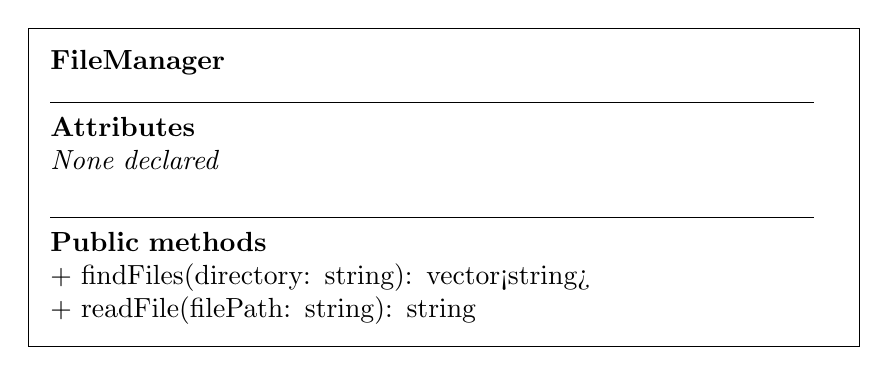
\begin{tikzpicture}\node[draw,rectangle,align=left,text width=10cm,inner sep=8pt] {
\textbf{FileManager}\\\rule{9.7cm}{0.4pt}\\
\textbf{Attributes}\\\emph{None declared}\\[2mm]\rule{9.7cm}{0.4pt}\\
\textbf{Public methods}\\+ findFiles(directory: string): vector<string>\\+ readFile(filePath: string): string};
\end{tikzpicture}\caption{UML class diagram for FileManager.}\end{figure}
\end{document}
